\begin{document}
	\chapter{Results}
	
	The study conducted over the data gathered served for the definition of new metrics to measure the performance and robustness of the Lightning Network and for the formal modeling of two mathematical representation of the Lightning Network, from a static and dynamic point of view. The analysis is carried over a period of one month, one snapshot per day; this observation period will be justified by the results obtained by the analysis of daily behavior of the network that will be shown next. 
	
	\section{Trends}
	
	The following section takes in consideration the most relevant trends of the network which are the nodes and edges variation, the average degree and the diameter of the network on a daily and a monthly basis. The analysis carried over the daily basis data is made to justify the decision of the focus on a larger time window. 
	
	A full day representation of the Lightning Network consists of 144 snapshots taken at 10 minutes intervals; the 10 minutes intervals were chosen because every channel that is added (or removed) from the network must wait for the funding transaction (settlement transaction in case a channel is being closed) to be included in a block and added to the chain by the miners. The following results matched the expectation because, as stated in the white paper, a Lightning node and its channels are meant to have a long lifespan. The data refers to the date of 16th of May, 21th of May ,26th of May, 2nd of June, 
	
	\subsection{Daily nodes variation}
	
	\begin{figure}[h]
		\centering
		\begin{subfigure}{0.45\textwidth}
			\centering
			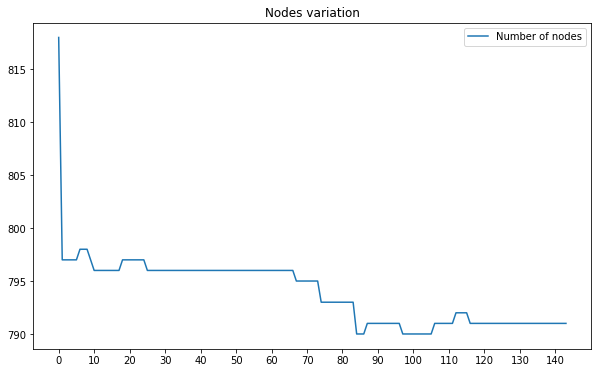
\includegraphics[width=\linewidth]{daily_number_of_nodes0}
		\end{subfigure}
		\begin{subfigure}{0.45\textwidth}
			\centering
			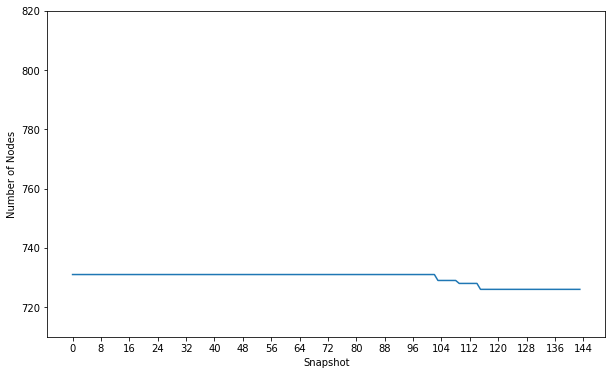
\includegraphics[width=\linewidth]{daily_number_of_nodes1}
		\end{subfigure}
			\begin{subfigure}{0.45\textwidth}
			\centering
			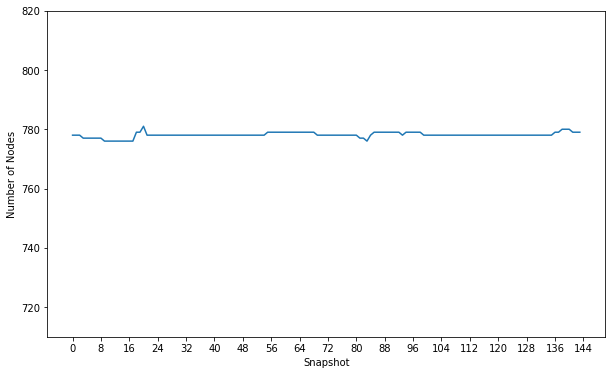
\includegraphics[width=\linewidth]{daily_number_of_nodes2}
		\end{subfigure}
		\begin{subfigure}{0.45\textwidth}
			\centering
			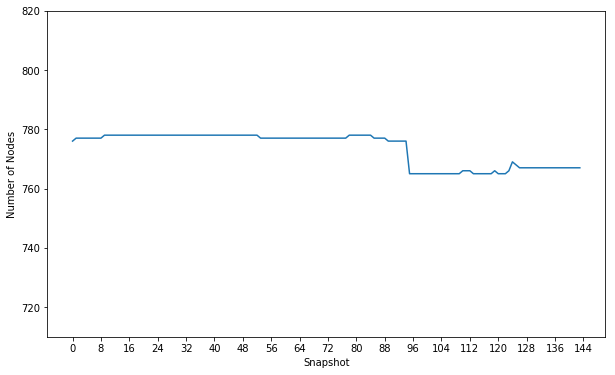
\includegraphics[width=\linewidth]{daily_number_of_nodes3}
		\end{subfigure}
		
		\caption{Nodes variation on a daily basis}
		\label{daily_nodes_variation}
	\end{figure}

	Details on nodes variations on a daily basis are reported in \ref{daily_nodes_variation}. The figure shows the 144 snapshot of the network for four different days. 
	\subsection{Daily edges variation}
	\subsection{Daily average degree variation}
	\subsection{Daily diameter}
	\subsection{Daily average eccentricity}
	\subsection{Weekly nodes variation}
	\subsection{Weekly edges variation}
	\subsection{Weekly average degree variation}
	\subsection{Weekly diameter}
	\subsection{Weekly average eccentricity}
	\section{Betwenness	 centrality}
	\subsection{Daily betweenness centrality - top 5}
	\subsection{Gantt chart - day}
	\subsection{Weekly betweenness centrality - top 5}
	\subsection{Gantt chart - week}
	\section{\textit{k}-vertex connectivity}
	\subsection{Components size}
	\subsection{Betweenness inclusion}
	\section{Max-Cut}
\end{document}